% Drawing 104/01-1 -- folder 104, batch 01, archive page 1 (PDF page 2).
% Transcription: moitié supérieure du feuillet, quatre rangées de figures (complexes cellulaires esquissés). Première rangée : trois segments portant trois, quatre puis cinq marques de subdivision (extrémités comprises). Deuxième rangée : un petit rectangle divisé en deux ; une amande hachurée coupée par son grand axe ; deux amandes hachurées accolées par une pointe, avec dessous un petit rectangle divisé en deux. Troisième rangée : une bande verticale de trois carrés ; une amande hachurée fermée en dessous par un second arc (un disque à deux étages) ; trois amandes hachurées accolées en chaîne, la première raturée en son milieu, avec dessous un rectangle divisé en trois. Quatrième rangée : un huit (deux cercles tangents en un point) traversé par une horizontale, et un petit carré divisé en quatre. Deux longues courbes séparent les groupes.
% Kind: rows of sketched cell complexes: subdivided segments, hatched almonds, divided squares, a figure of eight. Method 2 (schematic redraw from the facsimile). Status: partial.
% Notes: All the figures of the upper half of the sheet, each redrawn at its place: three segments with 3, 4 and 5 subdivision marks (ends included; each mark computed on its segment); the small rectangle cut in two; the hatched almond with its long axis; the pair of hatched almonds sharing one tip (drawn through the same point), with the small rectangle cut in two under them; the vertical strip of three squares; the almond with a second arc below it, hatched; the chain of three hatched almonds, consecutive ones sharing a tip, with the rectangle cut in three under them; the figure of eight (two circles through one common point) with the horizontal line through that point; the small square cut in four; the two long curves that separate the groups. Left out: the scribble that strikes the middle of the first almond of the chain (struck material). Still differs: the almonds and their hatching are regularised (his hatching strokes are free, 3 to 5 per almond); the two separating curves are smooth curves through points read on the crop. Disagreement in part with the note of the transcription, which counts « deux, trois puis quatre marques de subdivision »: the three segments carry 3, 4 and 5 marks counting their ends (1, 2 and 3 inner marks). Overlaid on the 400 dpi colour facsimile on 2026-11-12 (Opus 5.5): every figure lies on the page within about 1 mm; not changed. What is listed above as regularised still is. Redrawn 2026-11-12 (issue 128): to check again. 2026-11-13, Claude Opus 5.5, overlay check (issue 147): laid over the scan rendered at 350 dpi in colour; not compiled (no TeX engine in the session), the TikZ was rasterised by a script; nothing changed. The segments, rectangles, the strip of squares, the small square cut in four, the outlines of the almonds and the two separating curves lie on their ink within about 1 unit. Kept partial for what is still regularised: the hatching of the almonds and of the disc is drawn as even strokes, not his free strokes (3 to 5 an almond, at their own slants); the second arc under the almond of the third row ends lower than his; the two circles of the figure of eight are drawn round where his are slightly flattened (up to 1 unit off at the bottom).
% Coordinates: 1 unit = 1 mm = 1/100 of the crop width (bbox in page fractions: [0.11, 0.075, 0.64, 0.285]).
% Redrawn by Claude (claude-fable-5-2), issue #128, 2026-11-12; not checked by a human; not compiled (no TeX in the session).
% Checked by Claude (claude-opus-5-5) 2026-11-12 (issue #128): overlaid on the 400 dpi colour facsimile; matches as far as the notes say. Not compiled. Status: partial.
% Rights: reproduces part of the work -- behind RENDER_TRANSCRIPTS, never published by itself.
\documentclass[tikz,border=3pt]{standalone}
\usepackage{amsmath,amssymb}
\usetikzlibrary{patterns,arrows.meta}
\tikzset{pencil/.style={black!45}, struck/.style={black!35}, mpt/.style={circle,draw,inner sep=1.3pt}, pt/.style={circle,fill,inner sep=0.9pt}, opt/.style={circle,draw,fill=white,inner sep=1.1pt}}
\begin{document}
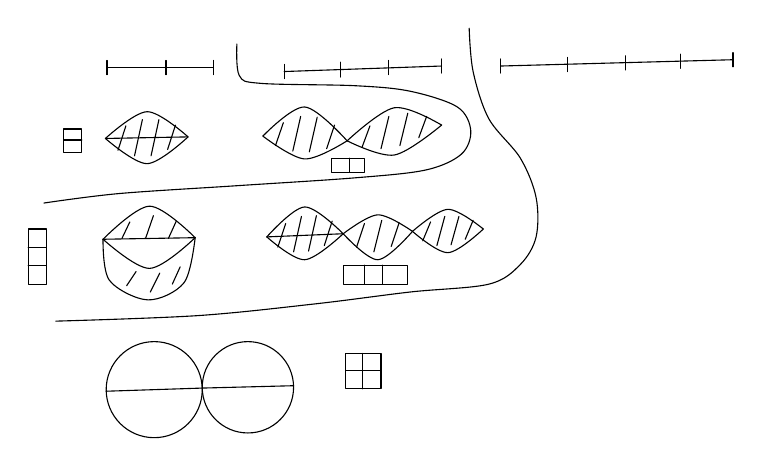
\begin{tikzpicture}[x=1mm,y=1mm,line cap=round,line join=round,font=\scriptsize]
\draw (13.5,-7.5) -- (27,-7.5);
\draw (13.5,-6.6) -- (13.5,-8.4);
\draw (21,-6.6) -- (21,-8.4);
\draw (27,-6.6) -- (27,-8.4);
\draw (36,-8) -- (56,-7.3);
\draw (36,-7.1) -- (36,-8.9);
\draw (43.2,-6.8) -- (43.2,-8.7);
\draw (49.3,-6.6) -- (49.3,-8.4);
\draw (56,-6.4) -- (56,-8.2);
\draw (63.5,-7.3) -- (93,-6.5);
\draw (63.5,-6.4) -- (63.5,-8.2);
\draw (72,-6.2) -- (72,-8);
\draw (79.3,-6) -- (79.3,-7.8);
\draw (86.3,-5.8) -- (86.3,-7.6);
\draw (93,-5.6) -- (93,-7.4);
\draw plot[smooth, tension=0.55] coordinates {(30,-4.5) (30.3,-8.5) (33,-9.5) (45,-9.8) (52,-10.5) (58,-12.5) (59.7,-15.5) (58.5,-18.5) (54,-20.5) (45,-21.5) (30,-22.5) (15,-23.5) (5.5,-24.7)};
\draw plot[smooth, tension=0.55] coordinates {(59.5,-2.5) (60,-8) (62,-14) (66,-19) (68,-24) (68,-29) (66,-32.5) (62,-35) (52,-36) (40,-37.5) (25,-39) (7,-39.7)};
\draw (8,-15.3) -- (10.3,-15.3) -- (10.3,-18.3) -- (8,-18.3) -- cycle;
\draw (8,-16.7) -- (10.3,-16.7);
\draw plot[smooth, tension=0.55] coordinates {(13.3,-16.5) (18.6,-13.1) (23.8,-16.3)};
\draw plot[smooth, tension=0.55] coordinates {(13.3,-16.5) (18.6,-19.7) (23.8,-16.3)};
\draw (13.3,-16.5) -- (23.8,-16.3);
\draw (15.9,-14.9) -- (14.9,-18);
\draw (18,-14.1) -- (17,-18.7);
\draw (20.1,-14.1) -- (19.1,-18.7);
\draw (22.2,-14.8) -- (21.2,-17.9);
\draw plot[smooth, tension=0.55] coordinates {(33.3,-16.2) (38.6,-12.5) (44,-16.8)};
\draw plot[smooth, tension=0.55] coordinates {(33.3,-16.2) (38.6,-19.1) (44,-16.8)};
\draw (35.9,-14.5) -- (34.9,-17.4);
\draw (38.1,-13.7) -- (37.1,-18.1);
\draw (40.2,-13.8) -- (39.2,-18.2);
\draw (42.4,-14.8) -- (41.4,-17.8);
\draw plot[smooth, tension=0.55] coordinates {(44,-16.8) (50,-12.6) (56,-14.8)};
\draw plot[smooth, tension=0.55] coordinates {(44,-16.8) (50,-18.6) (56,-14.8)};
\draw (46.9,-14.9) -- (45.9,-17.6);
\draw (49.3,-13.7) -- (48.3,-17.8);
\draw (51.7,-13.3) -- (50.7,-17.4);
\draw (54.1,-13.7) -- (53.1,-16.4);
\draw (42,-19) -- (46.2,-19) -- (46.2,-20.8) -- (42,-20.8) -- cycle;
\draw (44.3,-19) -- (44.3,-20.8);
\draw (3.5,-28) -- (5.8,-28) -- (5.8,-35) -- (3.5,-35) -- cycle;
\draw (3.5,-30.3) -- (5.8,-30.3);
\draw (3.5,-32.6) -- (5.8,-32.6);
\draw plot[smooth, tension=0.55] coordinates {(13,-29.3) (18.9,-25.1) (24.7,-29.1)};
\draw plot[smooth, tension=0.55] coordinates {(13,-29.3) (18.9,-33) (24.7,-29.1)};
\draw (13,-29.3) -- (24.7,-29.1);
\draw (16.4,-27.1) -- (15.4,-29.2);
\draw (19.4,-26.3) -- (18.4,-29.2);
\draw (22.3,-27) -- (21.3,-29.2);
\draw plot[smooth, tension=0.55] coordinates {(13,-29.3) (13.8,-34.5) (18.7,-37) (23.3,-34.8) (24.7,-29.1)};
\draw (16,-35.2) -- (17.2,-33.4);
\draw (19,-36) -- (20.2,-33.6);
\draw (21.8,-35) -- (22.8,-32.8);
\draw plot[smooth, tension=0.55] coordinates {(33.8,-29) (38.6,-25.2) (43.5,-28.6)};
\draw plot[smooth, tension=0.55] coordinates {(33.8,-29) (38.6,-31.9) (43.5,-28.6)};
\draw (33.8,-29) -- (43.5,-28.6);
\draw (36.2,-27.3) -- (35.2,-30.3);
\draw (38.2,-26.4) -- (37.2,-30.9);
\draw (40.1,-26.3) -- (39.1,-30.8);
\draw (42.1,-27) -- (41.1,-30.1);
\draw plot[smooth, tension=0.55] coordinates {(43.5,-28.6) (47.9,-26.2) (52.3,-28.3)};
\draw plot[smooth, tension=0.55] coordinates {(43.5,-28.6) (47.9,-31.9) (52.3,-28.3)};
\draw (46.2,-27.3) -- (45.2,-30.3);
\draw (48.4,-26.9) -- (47.4,-30.9);
\draw (50.6,-27.2) -- (49.6,-30.2);
\draw plot[smooth, tension=0.55] coordinates {(52.3,-28.3) (56.8,-25.5) (61.3,-28)};
\draw plot[smooth, tension=0.55] coordinates {(52.3,-28.3) (56.8,-31) (61.3,-28)};
\draw (54.6,-27.1) -- (53.6,-29.5);
\draw (56.4,-26.4) -- (55.4,-30.1);
\draw (58.2,-26.4) -- (57.2,-30);
\draw (60,-26.9) -- (59,-29.3);
\draw (43.5,-32.6) -- (51.7,-32.6) -- (51.7,-35) -- (43.5,-35) -- cycle;
\draw (46.2,-32.6) -- (46.2,-35);
\draw (48.5,-32.6) -- (48.5,-35);
\draw (19.5,-48.4) circle[radius=6.1];
\draw (31.4,-48.1) circle[radius=5.8];
\draw (13.4,-48.6) -- (25.6,-48.2) -- (37.2,-47.9);
\draw (43.8,-43.8) -- (48.3,-43.8) -- (48.3,-48.3) -- (43.8,-48.3) -- cycle;
\draw (46,-43.8) -- (46,-48.3);
\draw (43.8,-46) -- (48.3,-46);
\end{tikzpicture}
\end{document}
